En este capítulo, hablaremos de algunas herramientas y paquetes de Python que existen actualmente para garantizar la equidad en aprendizaje automático. Hablaremos de algunos de los más influyentes, entre los que destacaremos Aequitas. 

\section{Paquetes de Python para equidad en AA}

\section*{Ethik}

Ethik es un paquete de Python para realizar estudios sobre equidad en aprendizaje automático y obtener explicaciones sobre la misma. Ethik, utiliza el enfoque de la equidad contrafactual para dar solución a escenarios hipotéticos de injusticia en una población concreta. El paquete contiene una recopilación de conjuntos de datos sobre problemas de equidad a partir de la cual hemos podido extraer el \textit{dataset} denominado law\_data.csv que contiene el problema del Apartado \ref{subsec:desproblem} usando la función \textit{load\_law\_school()}.

Podemos encontrar la documentación y herramientas que proporciona el paquete en el siguiente enlace: \url{https://xai-aniti.github.io/ethik/}

\section*{Fairlearn}

Fairlearn es un paquete de Python que permite a los científicos de datos y desarrolladores de aplicaciones de \textit{machine learning} evaluar la equidad de su sistema y mitigar cualquier problema de sesgo en una población para un conjunto de datos observado. Fairlearn contiene  algoritmos de mitigación, así como métricas para la evaluación del modelo.

Podemos encontrar la documentación y guía de uso del paquete en el siguiente enlace: \url{https://fairlearn.org/v0.5.0/user_guide/index.html}

\section{Aequitas}

\textcolor{red}{NO REVISAR: Se completará con los experimentos usando la biblioteca de Aequitas}

Aequitas (\cite{aequitas2019}) es una herramienta de auditoría desarrollada por el \textit{Center for Data Science and Public Policy} de la
Universidad de Chicago. Es una herramienta de código abierto que consta de diversas utilidades de soporte para la auditoría de sesgos creado para ser utilizado por analistas de todo tipo relacionados con el ámbito del aprendizaje automático y cuyo principal objetivo es auditar los modelos de \textit{machine learning} con el fin de encontrar posibles discriminaciones en ellos y evitarlas en un futuro.

Aequitas nos permite detectar dos tipos de sesgos:

\begin{itemize}
    \item Acciones sesgadas que no ocurren de forma representativa en la población.
    \item Resultados sesgados a causa de errores de clasificación de nuestro sistema con respecto a ciertos grupos de la población.
\end{itemize}

Para utilizar la herramienta, se necesitan aportar los siguientes datos:

\begin{itemize}
    \item Datos sobre los atributos específicos (raza, sexo, etc.) que queramos auditar.
    \item El conjunto de personas de la población mencionada que el sistema de evaluación de riesgos seleccionó para una intervención.
\end{itemize}

\subsection*{Estructura de los datos de entrada y resultados}

Podemos dividir en tres apartados (conformados por columnas en Aequitas) los datos que debemos aportar para el correcto funcionamiento de la herramienta.

\begin{itemize}
    \item \textbf{score}: representa la conclusión a la que llega un modelo, puede ser puede ser binaria ($0$ o $1$) o continua (decimal entre $0$ y $1$). Esta decisión representa si el sujeto es apto o no, por ejemplo, si se le concede un crédito bancario.
    \item \textbf{label\_value}: representa los datos reales, es decir, si la predicción realizada por el modelo fue correcta. Por ejemplo, el sujeto fue capaz de devolver el crédito en su totalidad. Es por esto, por lo que el modelo solo puede ser auditado después de su aplicación y no antes. Se representa como un valor binario, $1$ significa que la predicción fue correcta, $0$ que no lo fue.
    \item \textbf{attributes}: categorías de los atriburtos definidos por el usuario y utilizados para decidir la equidad del modelo. Algunos ejemplos de atributos son la raza, sexo, educación, edad o ingresos.
\end{itemize}

El funcionamiento de Aequitas viene determinado por los conceptos y métricas definidas previamente en la Sección \ref{sec:groupmetrics}. Podemos acceder a una lista de los conceptos y métricas que utiliza Aequitas a partir del siguiente enlace: \url{https://dssg.github.io/aequitas/metrics.html}

La herramienta devuelve una interpretación gráfica de los resultados junto a información relevante acerca de tres tipos de métricas:

\begin{itemize}
    \item Métricas de grupo.
    \item Métricas de sesgo.
    \item Medidas de equidad.
\end{itemize}

A continuación mostraremos dos ejemplos de uso de Aequitas utilizando por un lado la herramienta de la aplicación WEB y por otro la API de Python que incluye un mayor número de métricas y gráficas para interpretar los resultados.

\subsection{Ejemplo: Puntuación del riesgo de reincidencia delictiva}

A continuación, analizaremos como se definen las diferentes métricas con las que trabaja Aequitas a partir de los conceptos previamente estudiados. Mostraremos un ejemplo sobre el conjunto de datos \textit{COMPAS} cuyo objetivo era identificar a las personas con riesgo de reincidencia para respaldar las decisiones de liberación previa al juicio.\\

\begin{table}[h]
\centering
\resizebox{12.4cm}{!} {
\begin{tabular}{|c|c|c|c|c|}
\hline
\textbf{score} & \textbf{label\_value} & \textbf{race}    & \textbf{sex} & \textbf{age\_cat} \\ \hline
0             & 1                     & Hispanic & Male       & Less than 25             \\ \hline
1              & 0                     & African-American         & Female         & 25-45     \\ \hline
0              & 0                     & Caucassian       & Male         & 25-45            \\ \hline
\end{tabular}
}
\caption{Ejemplo del \textit{dataset COMPAS} aportado a Aequitas.}
\label{tab:ejcompasaeq}
\end{table}

Los datos están basados en las estadísticas recogidas en el condado de Broward y puestas a disposición del público por la organización ProPublica (\cite{condena2016}). Este conjunto de datos contiene una puntuación del riesgo de reincidencia para 7.214 individuos, sus resultados reales de reincidencia a los dos años y una serie de atributos recogidos entre 2013 y 2014.

\subsection*{Métricas de grupo}

Primero calcularemos una tabla con los valores de las métricas de grupo para un atributo concreto (p.ej. raza) y tomaremos como atributo de referencia la raza \textit{Caucassian}. 

En nuestro caso la raza \textit{Caucassian} no es la raza mayoritaria en el conjunto de datos, pero la tomaremos como referencia debido a que históricamente en el ámbito en el que nos movemos es la que sufre menos sesgos.\\

\begin{figure}[h]
	\centering
	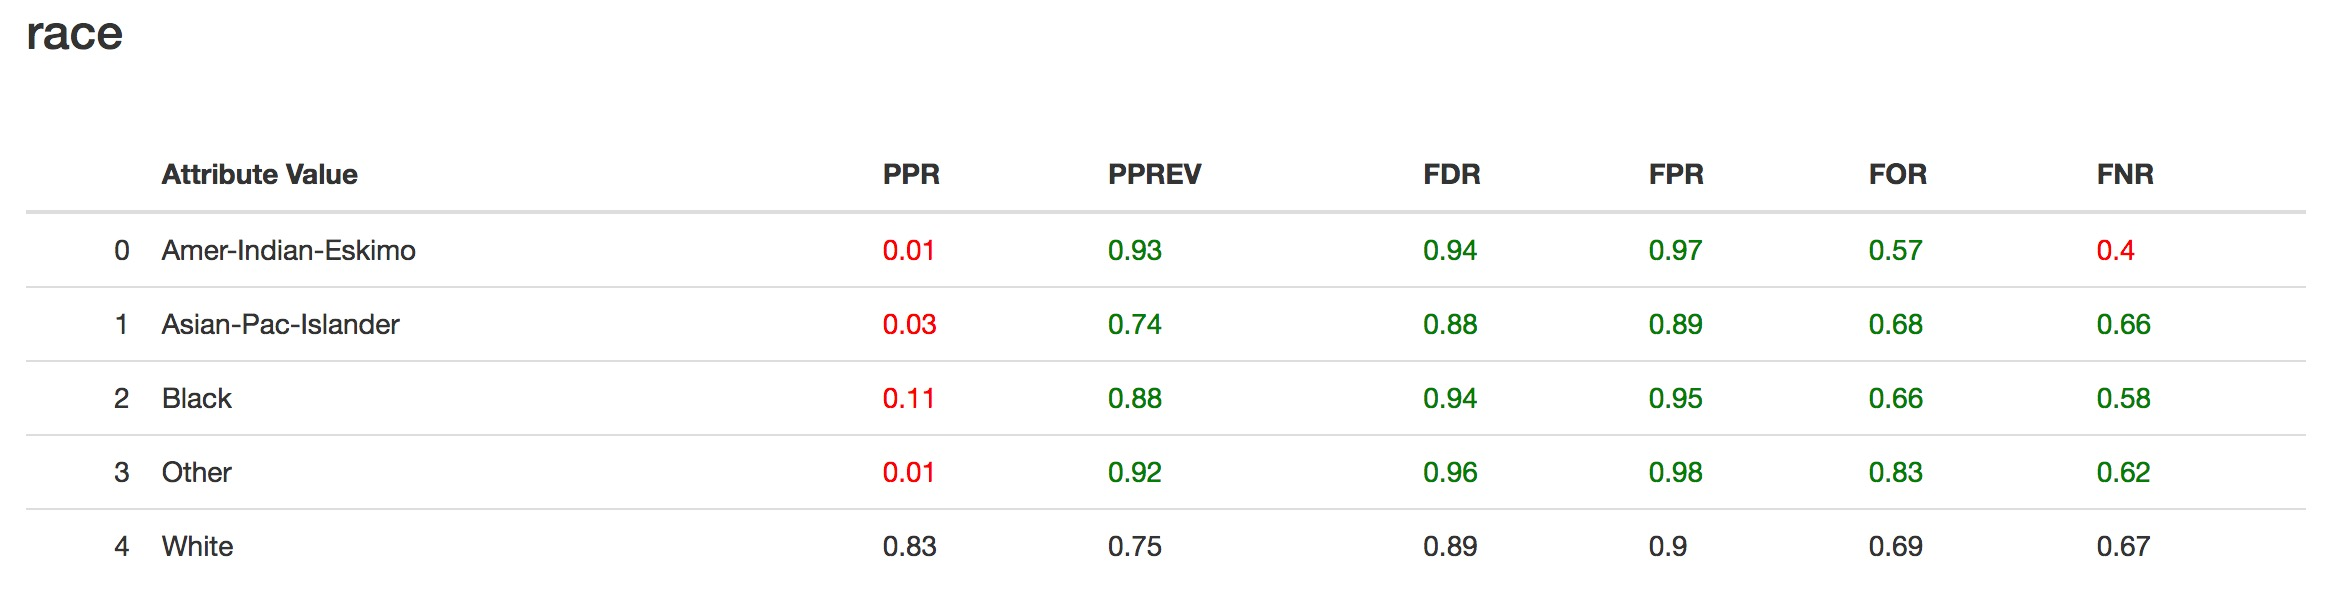
\includegraphics[width=16.7cm]{group_adult_aq.jpg}
	\caption{Tabla con las principales métricas de grupo para el atributo \textit{race}.}
    \label{fig:ejaq1}
\end{figure}

\subsection*{Métricas de sesgo}

A continuación mediremos la disparidad entre cada grupo objetivo y el grupo de referencia seleccionado. Aequitas calcula la disparidad a partir de la fórmula que ya definimos en el Apartado \ref{subsec:impactdesi}. $$\text{Métrica de disparidad}_{G(a_o)}=\ddfrac{\text{Métrica}_{a_o}}{\text{Métrica}_{a_r}}.$$ Donde Métrica hace referencia a una métrica de grupo de la Sección \ref{sec:groupmetrics}. Es evidente que la disparidad de cualquier métrica sobre el grupo de referencia será 1. $$\text{Métrica de disparidad}_{G(a_r)}=\ddfrac{\text{Métrica}_{a_r}}{\text{Métrica}_{a_r}}=1.$$

Si queremos calcular por ejemplo la disparidad del ratio de falsos negativos (FNR) sobre el grupo de raza \textit{Asian}, se calculará de la siguiente forma: $$\text{FNR}_{\text{G(Asian)}}=\ddfrac{\text{FNR}_{\text{Asian}}}{\text{FNR}_{\text{Caucassian}}}=\ddfrac{0.33}{0.48}=0.7.$$

Para ver otro ejemplo de cómo realiza el cálculo Aequitas, mediremos la disparidad para la tasa de falso descubrimiento (FDR) sobre el grupo de raza \textit{Hispanic}:
$$\text{FDR}_{\text{G(Hispanic)}}=\ddfrac{\text{FDR}_{\text{Hispanic}}}{\text{FDR}_{\text{Caucassian}}}=\ddfrac{0.3}{0.35}=0.86.$$

Completando la tabla con las métricas de disparidad para todas las métricas de grupo obtendremos el siguiente resultado:\\

\begin{figure}[h]
	\centering
	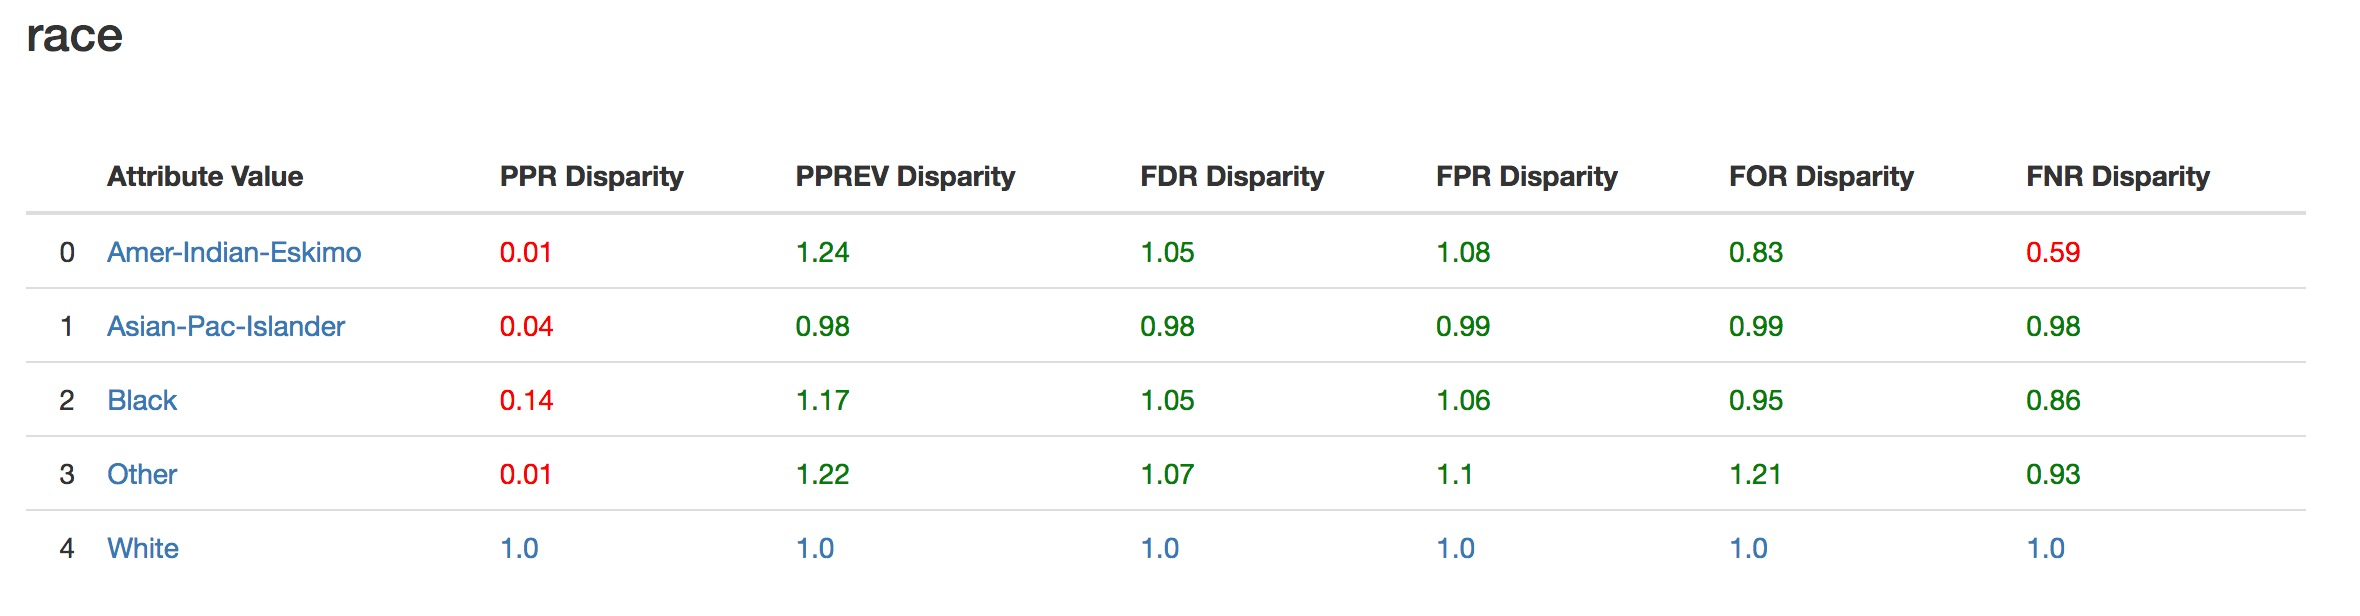
\includegraphics[width=16.7cm]{disparity_adult_aq.jpg}
	\caption{Tabla con las métricas de sesgo para el atributo \textit{race} con umbral del 80\%.}
    \label{fig:ejaq2}
\end{figure}

\subsection*{Medidas de equidad}

La equidad siempre se define en relación con un grupo de referencia. Podemos ver que el cálculo de la equidad, depende de la métrica de sesgo. En la evaluación del criterio de equidad definiremos un $\epsilon \in [0,1)$ como umbral de equidad. Diremos que un grupo cumple con la paridad métrica si $$1-\epsilon\leq \text{\text{Métrica de disparidad}}_{\text{G}} \leq \ddfrac{1}{1-\epsilon}.$$

En nuestro ejemplo, hemos tomando $\epsilon=0.2$ por lo que cualquier métrica de sesgo se considerará justa si se está contenida en el intervalo $$\left[1-0.2,\ddfrac{1}{1-0,2}\right]=[0.8,1.25].$$

En la Figura \ref{fig:ejaq2}, vemos en verde los valores contenidos en el intervalo y en rojo, los que se encuentran fuera del mismo. En los resultados finales, si para todos los atributos existe una métrica de disparidad que contiene todos sus valores en color verde, el modelo se evaluará como justo para esa métrica. De lo contrario, lo considerará injusto y enumerará los grupos afectados según los criterios de equidad dados.\\

\begin{figure}[h]
	\centering
	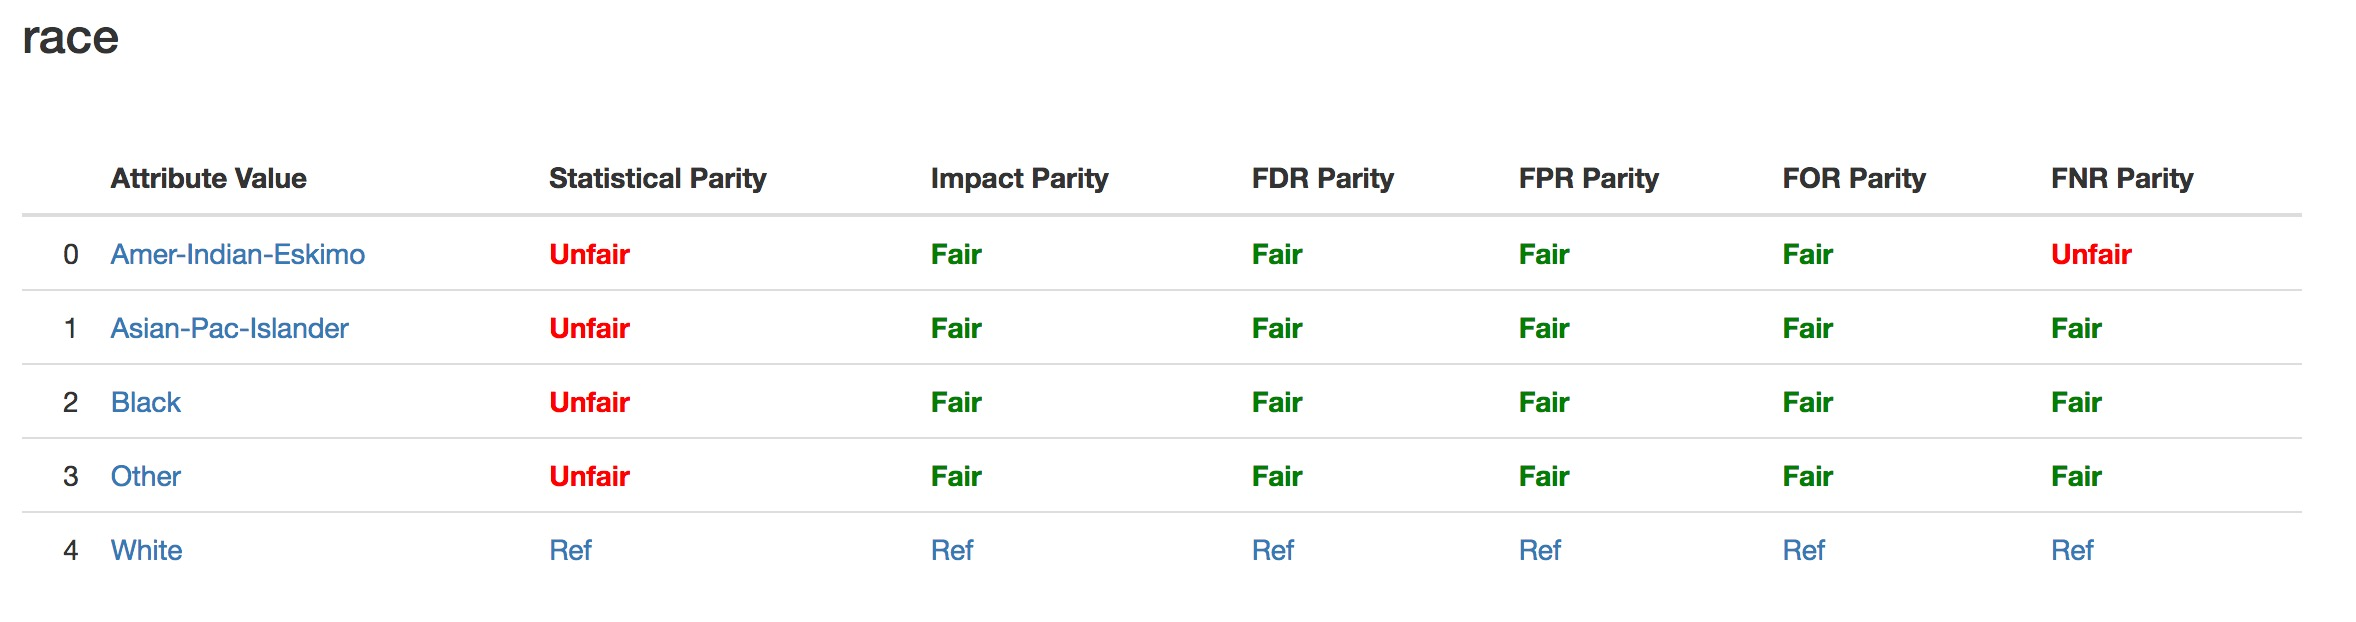
\includegraphics[width=16.7cm]{fairness_adult_output.jpg}
	\caption{Tabla de medidas de equidad aplicado el umbral del 80\%.}
    \label{fig:medequmbral}
\end{figure}

En nuestro ejemplo, estamos usando la regla del 80\% recomendada por la EEOC (\cite{adverse2009}) donde $p=1-\epsilon$ y por tanto $p=0.8$. En este caso, todas las métricas de disparidad aparecen como injustas, como podemos observar en la Figura \ref{fig:medequmbral}.\\

\begin{figure}[h]
	\centering
	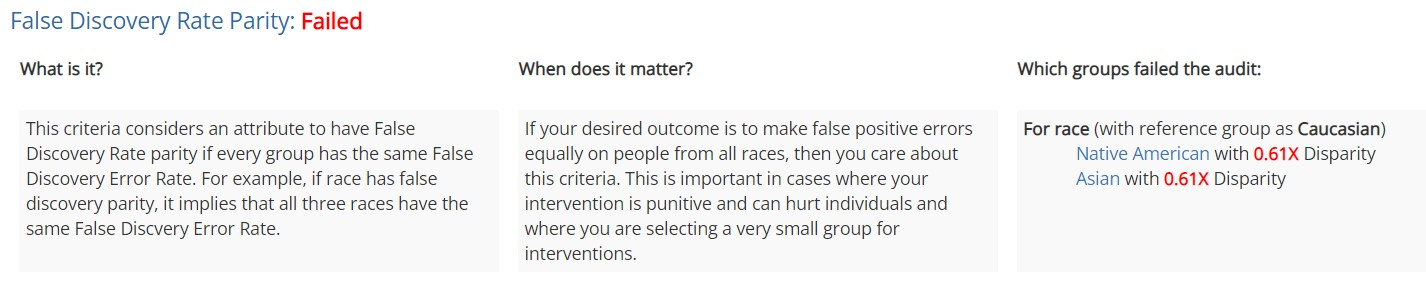
\includegraphics[width=16.7cm]{fairness_output_aq2.jpg}
	\caption{Resultado injusto para la paridad métrica FDR con $p=0.8$.}
    \label{fig:ejunfairaq2}
\end{figure}

Si cambiamos la ''regla p'' de un 80\% a, por ejemplo, un 60\% el intervalo del umbral para $p=0.6$ sería $[0.6,1.67]$ y obtenemos los siguientes resultados.

\begin{figure}[h]
	\centering
	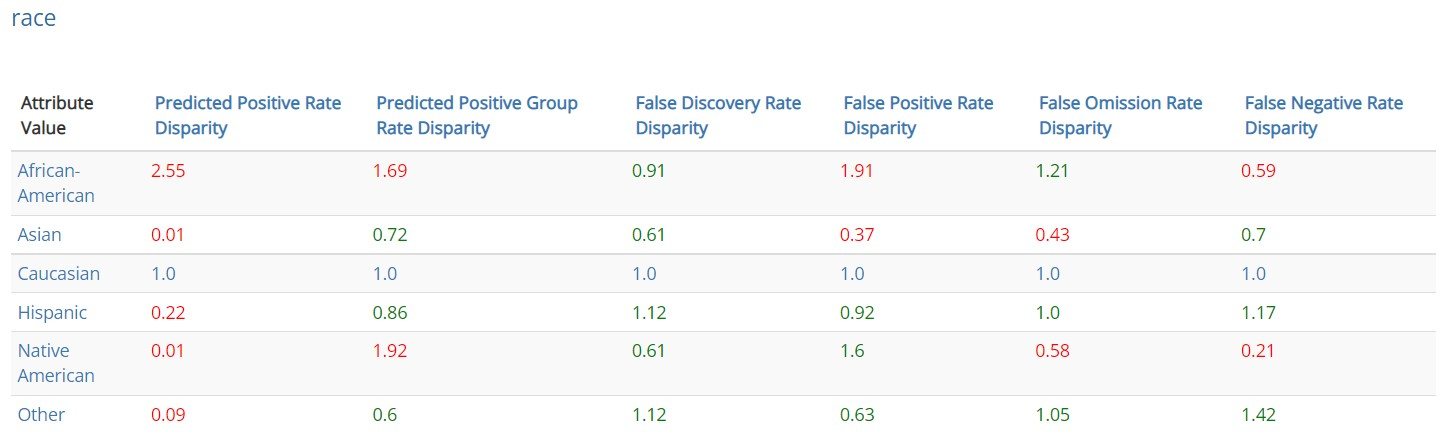
\includegraphics[width=16.7cm]{disparity_adult_aq2.jpg}
	\caption{Tabla con las métricas de sesgo para el atributo \textit{race} con $p=0.6$.}
    \label{fig:ejaq22}
\end{figure}

En la figura anterior podemos observar que la paridad de la tasa de falso descubrimiento (FDR) se se acepta como justa. Aequitas nos ofrece una breve descripción en este caso de la métrica justa.\\

\begin{figure}[h]
	\centering
	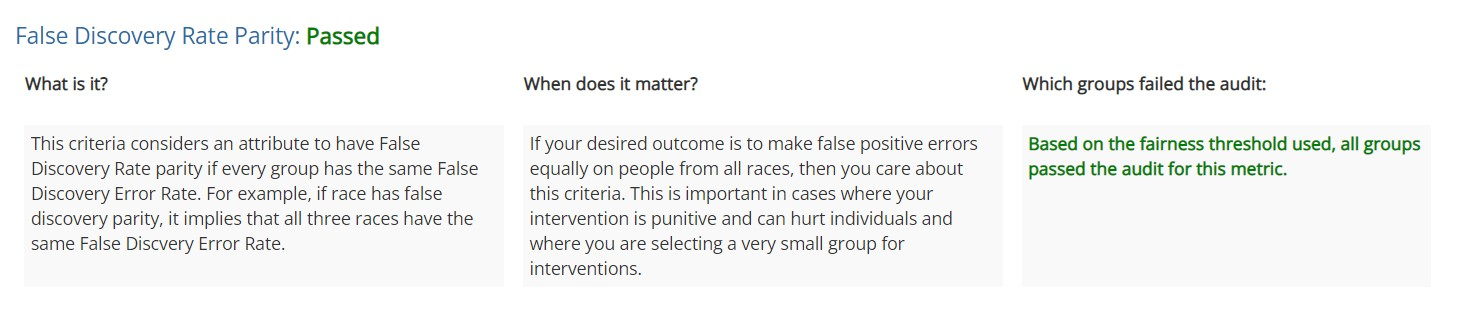
\includegraphics[width=16.7cm]{fairness_output_aq.jpg}
	\caption{Resultado justo para la paridad métrica FDR con $p=0.6$.}
    \label{fig:ejunfairaq}
\end{figure}



\textcolor{red}{La versión actual es un esquema de lo que se intentará mostrar con imágenes sacadas de la web que deben cambiarse. Idea probar en Aequitas con las medidas existentes el mismo dataset que usaré con contrafactual, si no se puede, usar COMPAS.}

\subsection{Ejemplo: Predicción de notas en la facultad de derecho}